{\Large \textbf{Partie I}}


\subsection*{Équations différentielles d'ordre 1 solubles par la séparation des variables}

\begin{enumerate}
\item $y' + 3t^2 y = 0$:

\[y' = -3t^2 y\]
\[\frac{y'}{y} = -3t^2\]

Intégrons par rapport à $dt$:

\[\int_0^x \frac{y'(t)}{y(t)} dt = -3\int_0^xt^2 dt \]
\[\ln(y(x)) - \ln(y(0)) = -x^3\]

On trouve que:

\[y(x) = 2e^{-x^3}\]


\item $yy' + t = 1$:

\[y(t)y'(t) = 1- t\]

Intégrons par rapport à $dt$:

\[\int_0^x y(x)y'(x)dx = \int_0^x(1-t) dt\]

\[\frac{1}{2}(y^2(x) - y^2(0)) = \frac{1}{2}(2x - x^2)\]

Donc:

\[y(x) = \sqrt{1 + 2x - x^2}\]


\item $(t^3 + 1)y' + t^2 y^2 = 0$:

\[\frac{y'}{y^2} = -\frac{t^2}{t^3 + 1}\]

Intégrons par rapport à $dt$:

\[\int_0^x\frac{y'(t)}{y^2(t)}dt = -\int_0^x\frac{t^2}{t^3 + 1}dt\]

\[\frac{1}{y(0)} - \frac{1}{y(x)} = -\frac{1}{3}\ln(x^3 + 1)\]

Donc:

\[y(x) = \frac{3}{3 + \ln(x^3 + 1)}\]
\end{enumerate}



\subsection*{Équation différentielle linéaire d'ordre 1 coefficients et second membre variables}

On a que $y'(t) + 4t^3y(t) = \exp(-t^4 + 2t)$, avec $y(0) = 1$.

Premièrement, pour l'équation homogène:

\[y_h'(t) + 4t^3y_h(t) = 0\]

\[\frac{y_h'}{y_h} = -4t^3\]

Donc:

\[\int \frac{y_h'}{y_h} dt = -\int4t^3dt\]

\[\ln(y_h(t)) = C - t^4\]

Pour une constante $C \in \R$, de façon que la solution générale homogène:

\[y_h(t) = C_1e^{-t^4}\]


Maintenant pour l'équation complète, il suffit de trouver une solution particulière $y_p(t)$ et ajouter la solution homogène.

Alors, supposons une solution particulière de la forme $y_p(t) = f(t) \cdot \exp(-t^4 + 2t)$. Ainsi, $y'_p(t) = \left[f'(t) + (-4t^3 + 2)f(t) \right]\cdot \exp(-t^4 + 2t)$. Donc, en appliquant dans l'équation:

\[\left[f'(t) + 2f(t) \right]\cdot \exp(-t^4 + 2t) = \exp(-t^4 + 2t)\]

\[\implies f'(t) + 2f(t) = 1\]

Comme nous voulons trouver une solution quelconque pour $y_p(t)$ on peut prendre la solution plus simple de $f(t)$:

\[f(t) = \frac{1}{2}\]

Donc $y_p(t) = \frac{1}{2}\exp(-t^4+2t)$. Maintenant pour la solution générale:

\[y(t) = C_1 e^{-t^4} + \frac{1}{2}e^{-t^4 + 2t}\]

Pour que $y(0) = 1$ il faut que $C_1 = \frac{1}{2}$:

\[\therefore y(t) = \frac{1}{2}(1 + e^{2t})e^{-t^4}\]


\subsection*{Équation différentielle linéaire d'ordre 2 coefficients et second membre variables}

Pour la solution homogène:

\[y_h''(t) - 5y_h'(t) + 6y_h(t) = 0\]

Le polynôme caractéristique est $x^2 - 5x + 6$, dont les racines sont $x_1 = 2$ et $x_2 = 3$, de façon que:

\[y_h(t) = C_1e^{2t} + C_2e^{3t}\]

Maintenant il faut trouver une solution particulière $y_p(t)$. Si l'on dérive $te^t$, il y aura des termes de $e^t$ et $te^t$, alors, supposons $y_p(t) = a \cdot e^t + b \cdot te^t$:

\[y_p'(t) = (a+b)e^t + bte^t\]
\[y_p''(t) = (a+2b)e^t + bte^t\]

De façon que:

\[(2a-3b)e^t + (2b)te^t = te^t\]

Donc $b = \frac{1}{2}$ et $a = \frac{3}{4}$:

\[y_p(t) = \frac{3 + 2t}{4}e^t\]

\[\therefore y(t) = C_1e^{2t} + C_2e^{3t} + \frac{3 + 2t}{4}e^t\]

Comme $y(0) = 0$ et $y'(0) = 0$, on arrive que $C_1 = -1$ et $C_2 = \frac{1}{4}$.

\[y(t) = -e^{2t} + \frac{1}{4}e^{3t}+ \frac{3 + 2t}{4}e^t\]



{\Large \textbf{Partie II}}

\begin{enumerate}
\item Considérons la figure:


\begin{center}
\tikzset{every picture/.style={line width=0.75pt}} %set default line width to 0.75pt        

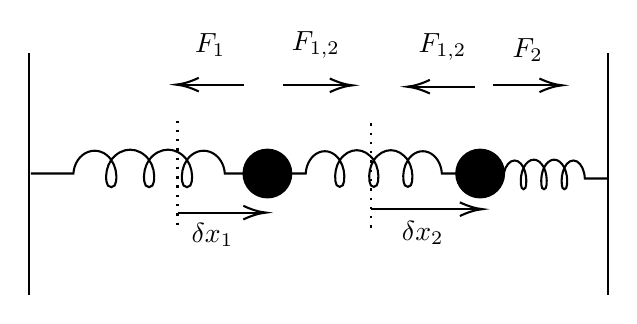
\begin{tikzpicture}[x=0.75pt,y=0.75pt,yscale=-1,xscale=1]
	%uncomment if require: \path (0,435); %set diagram left start at 0, and has height of 435
	
	%Straight Lines [id:da8139997984603213] 
	\draw    (200,108.5) -- (200,225) ;
	%Straight Lines [id:da07019762619638148] 
	\draw    (479,108.5) -- (479,225) ;
	%Shape: Circle [id:dp7624157630559317] 
	\draw  [fill={rgb, 255:red, 0; green, 0; blue, 0 }  ,fill opacity=1 ] (303.5,166.5) .. controls (303.5,160.15) and (308.65,155) .. (315,155) .. controls (321.35,155) and (326.5,160.15) .. (326.5,166.5) .. controls (326.5,172.85) and (321.35,178) .. (315,178) .. controls (308.65,178) and (303.5,172.85) .. (303.5,166.5) -- cycle ;
	%Shape: Circle [id:dp8917031379948387] 
	\draw  [fill={rgb, 255:red, 0; green, 0; blue, 0 }  ,fill opacity=1 ] (406,166.5) .. controls (406,160.15) and (411.15,155) .. (417.5,155) .. controls (423.85,155) and (429,160.15) .. (429,166.5) .. controls (429,172.85) and (423.85,178) .. (417.5,178) .. controls (411.15,178) and (406,172.85) .. (406,166.5) -- cycle ;
	%Shape: Inductor (Air Core) [id:dp1543763567402443] 
	\draw   (201,166.5) -- (221.52,166.5) .. controls (221.82,161.65) and (224.66,157.5) .. (228.69,156.05) .. controls (232.73,154.6) and (237.12,156.14) .. (239.76,159.94) .. controls (241.8,162.9) and (242.63,166.72) .. (242.04,170.44) .. controls (242.04,171.89) and (241.02,173.06) .. (239.76,173.06) .. controls (238.5,173.06) and (237.48,171.89) .. (237.48,170.44) .. controls (236.89,166.72) and (237.72,162.9) .. (239.76,159.94) .. controls (242.13,156.79) and (245.43,155) .. (248.88,155) .. controls (252.33,155) and (255.63,156.79) .. (258,159.94) .. controls (260.04,162.9) and (260.87,166.72) .. (260.28,170.44) .. controls (260.28,171.89) and (259.26,173.06) .. (258,173.06) .. controls (256.74,173.06) and (255.72,171.89) .. (255.72,170.44) .. controls (255.13,166.72) and (255.96,162.9) .. (258,159.94) .. controls (260.37,156.79) and (263.67,155) .. (267.12,155) .. controls (270.57,155) and (273.87,156.79) .. (276.24,159.94) .. controls (278.28,162.9) and (279.11,166.72) .. (278.52,170.44) .. controls (278.52,171.89) and (277.5,173.06) .. (276.24,173.06) .. controls (274.98,173.06) and (273.96,171.89) .. (273.96,170.44) .. controls (273.37,166.72) and (274.2,162.9) .. (276.24,159.94) .. controls (278.88,156.14) and (283.27,154.6) .. (287.31,156.05) .. controls (291.34,157.5) and (294.18,161.65) .. (294.48,166.5) -- (315,166.5) ;
	%Shape: Inductor (Air Core) [id:dp5572474041515377] 
	\draw   (315,166.5) -- (333.45,166.5) .. controls (333.72,161.76) and (336.28,157.7) .. (339.9,156.28) .. controls (343.53,154.86) and (347.47,156.37) .. (349.85,160.08) .. controls (351.68,162.98) and (352.43,166.72) .. (351.9,170.35) .. controls (351.9,171.77) and (350.98,172.92) .. (349.85,172.92) .. controls (348.72,172.92) and (347.8,171.77) .. (347.8,170.35) .. controls (347.27,166.72) and (348.02,162.98) .. (349.85,160.08) .. controls (351.98,157) and (354.95,155.25) .. (358.05,155.25) .. controls (361.15,155.25) and (364.12,157) .. (366.25,160.08) .. controls (368.08,162.98) and (368.83,166.72) .. (368.3,170.35) .. controls (368.3,171.77) and (367.38,172.92) .. (366.25,172.92) .. controls (365.12,172.92) and (364.2,171.77) .. (364.2,170.35) .. controls (363.67,166.72) and (364.42,162.98) .. (366.25,160.08) .. controls (368.38,157) and (371.35,155.25) .. (374.45,155.25) .. controls (377.55,155.25) and (380.52,157) .. (382.65,160.08) .. controls (384.48,162.98) and (385.23,166.72) .. (384.7,170.35) .. controls (384.7,171.77) and (383.78,172.92) .. (382.65,172.92) .. controls (381.52,172.92) and (380.6,171.77) .. (380.6,170.35) .. controls (380.07,166.72) and (380.82,162.98) .. (382.65,160.08) .. controls (385.03,156.37) and (388.97,154.86) .. (392.6,156.28) .. controls (396.22,157.7) and (398.78,161.76) .. (399.05,166.5) -- (417.5,166.5) ;
	%Shape: Inductor (Air Core) [id:dp24856022284547719] 
	\draw   (417.5,168.89) -- (428.57,168.89) .. controls (428.73,165.06) and (430.27,161.79) .. (432.44,160.65) .. controls (434.62,159.5) and (436.98,160.72) .. (438.41,163.71) .. controls (439.51,166.05) and (439.96,169.06) .. (439.64,171.99) .. controls (439.64,173.13) and (439.09,174.06) .. (438.41,174.06) .. controls (437.73,174.06) and (437.18,173.13) .. (437.18,171.99) .. controls (436.86,169.06) and (437.31,166.05) .. (438.41,163.71) .. controls (439.69,161.23) and (441.47,159.82) .. (443.33,159.82) .. controls (445.19,159.82) and (446.97,161.23) .. (448.25,163.71) .. controls (449.35,166.05) and (449.8,169.06) .. (449.48,171.99) .. controls (449.48,173.13) and (448.93,174.06) .. (448.25,174.06) .. controls (447.57,174.06) and (447.02,173.13) .. (447.02,171.99) .. controls (446.7,169.06) and (447.15,166.05) .. (448.25,163.71) .. controls (449.53,161.23) and (451.31,159.82) .. (453.17,159.82) .. controls (455.03,159.82) and (456.81,161.23) .. (458.09,163.71) .. controls (459.19,166.05) and (459.64,169.06) .. (459.32,171.99) .. controls (459.32,173.13) and (458.77,174.06) .. (458.09,174.06) .. controls (457.41,174.06) and (456.86,173.13) .. (456.86,171.99) .. controls (456.54,169.06) and (456.99,166.05) .. (458.09,163.71) .. controls (459.52,160.72) and (461.88,159.5) .. (464.06,160.65) .. controls (466.23,161.79) and (467.77,165.06) .. (467.93,168.89) -- (479,168.89) ;
	%Straight Lines [id:da7550159946155199] 
	\draw    (272,185.33) -- (312.33,185.33) ;
	\draw [shift={(314.33,185.33)}, rotate = 180] [color={rgb, 255:red, 0; green, 0; blue, 0 }  ][line width=0.75]    (10.93,-3.29) .. controls (6.95,-1.4) and (3.31,-0.3) .. (0,0) .. controls (3.31,0.3) and (6.95,1.4) .. (10.93,3.29)   ;
	%Straight Lines [id:da5935899926338495] 
	\draw    (364.67,183.67) -- (416.67,183.67) ;
	\draw [shift={(418.67,183.67)}, rotate = 180] [color={rgb, 255:red, 0; green, 0; blue, 0 }  ][line width=0.75]    (10.93,-3.29) .. controls (6.95,-1.4) and (3.31,-0.3) .. (0,0) .. controls (3.31,0.3) and (6.95,1.4) .. (10.93,3.29)   ;
	%Straight Lines [id:da862076015559579] 
	\draw  [dash pattern={on 0.84pt off 2.51pt}]  (271.67,141) -- (271.67,193.83) ;
	%Straight Lines [id:da02721360481530155] 
	\draw  [dash pattern={on 0.84pt off 2.51pt}]  (365,142.33) -- (365,195.17) ;
	%Straight Lines [id:da6483629457584736] 
	\draw    (303.67,123.67) -- (273,123.67) ;
	\draw [shift={(271,123.67)}, rotate = 360] [color={rgb, 255:red, 0; green, 0; blue, 0 }  ][line width=0.75]    (10.93,-3.29) .. controls (6.95,-1.4) and (3.31,-0.3) .. (0,0) .. controls (3.31,0.3) and (6.95,1.4) .. (10.93,3.29)   ;
	%Straight Lines [id:da8208435340337296] 
	\draw    (322.67,124) -- (354,124) ;
	\draw [shift={(356,124)}, rotate = 180] [color={rgb, 255:red, 0; green, 0; blue, 0 }  ][line width=0.75]    (10.93,-3.29) .. controls (6.95,-1.4) and (3.31,-0.3) .. (0,0) .. controls (3.31,0.3) and (6.95,1.4) .. (10.93,3.29)   ;
	%Straight Lines [id:da5965539997399391] 
	\draw    (423.67,124) -- (455,124) ;
	\draw [shift={(457,124)}, rotate = 180] [color={rgb, 255:red, 0; green, 0; blue, 0 }  ][line width=0.75]    (10.93,-3.29) .. controls (6.95,-1.4) and (3.31,-0.3) .. (0,0) .. controls (3.31,0.3) and (6.95,1.4) .. (10.93,3.29)   ;
	%Straight Lines [id:da6315906447883408] 
	\draw    (415,124.67) -- (384.33,124.67) ;
	\draw [shift={(382.33,124.67)}, rotate = 360] [color={rgb, 255:red, 0; green, 0; blue, 0 }  ][line width=0.75]    (10.93,-3.29) .. controls (6.95,-1.4) and (3.31,-0.3) .. (0,0) .. controls (3.31,0.3) and (6.95,1.4) .. (10.93,3.29)   ;
	
	% Text Node
	\draw (277,189.07) node [anchor=north west][inner sep=0.75pt]    {$\delta x_{1}$};
	% Text Node
	\draw (378.33,188.07) node [anchor=north west][inner sep=0.75pt]    {$\delta x_{2}$};
	% Text Node
	\draw (278.67,97.4) node [anchor=north west][inner sep=0.75pt]    {$F_{1}$};
	% Text Node
	\draw (325.33,96.73) node [anchor=north west][inner sep=0.75pt]    {$F_{1,2}$};
	% Text Node
	\draw (386.33,97.4) node [anchor=north west][inner sep=0.75pt]    {$F_{1,2}$};
	% Text Node
	\draw (431.67,100.07) node [anchor=north west][inner sep=0.75pt]    {$F_{2}$};
	
\end{tikzpicture}

\end{center}

Pour l'expression de chaque force $F_1$, $F_{1, 2}$ et $F_2$, par rapport à la direction de l'image, on a que:

\[\begin{cases}
	F_1 = K\delta x_1 \\
	F_{1,2} = K(\delta x_2 - \delta x_1) \\
	F_2 = -K\delta x_2
\end{cases}\]

\item L'équation de mouvement pour $m_1$:

\[F_T = F_{1,2} - F_1 = -2K\delta x_1 + K \delta x_2 = m_1 \delta\ddot{x_1}\]

Et pour $m_2$:

\[F_T = F_2 - F_{1,2} = K\delta x_1 - 2K \delta x_2 = m_2 \delta\ddot{x_2}\]

 Ces équations sont similaires à celles d'un mouvement oscillatoire, de façon que l'unité de $K/m_{1,2}$ est $s^{-2}$, équivalant à unité de pulsation (ou fréquence) au carrée.
 
 \item On a que:
 
 \[\begin{pmatrix}
 	\delta\ddot{x_1} \\
 	\delta\ddot{x_2} 
 \end{pmatrix} = \frac{d^2}{dt^2}\begin{pmatrix}
 \delta x_1 \\
 \delta x_2 
 \end{pmatrix} = K\begin{pmatrix}
 -\frac{2}{m_1} && \frac{1}{m_1} \\
 \frac{1}{m_2} && -\frac{2}{m_2}
 \end{pmatrix}\begin{pmatrix}
 \delta x_1 \\
 \delta x_2 
 \end{pmatrix}\]
 
 De façon que, pour $v(t) = [\delta x_1(t), \delta x_2(t)]^T$:

 \[\frac{d^2}{dt^2}v(t) = Mv(t)\]
 
 
 \item On doit diagonaliser la matrice $M$, de façon que l'on trouvera les vecteurs propres $v_1$ et $v_2$, tels que:
 
 \[\begin{cases}
 	Mv_1 = \lambda_1 v_1 \\
 	Mv_2 = \lambda_2 v_2
 \end{cases}\]
 
 Pour ces vecteurs, la solution de l'équation différentielle est désaccouplé par chaque ligne.
 
 Pour trouver les valeurs et vecteurs propres, il faut calculer le polynôme caractéristique de $M$:
 
 \[C_M(x) = x^2 - \text{tr}(M) x + \det(M)\] 
 \[C_M(x) = x^2 - 2K\frac{m_1+m_2}{m_1m_2}x + \frac{3K^2}{m_1m_2}\]
 
 Les racines de $C_M(x)$ sont:
 
 \[x_{1,2} = -\frac{K}{m_1m_2}\left(m_1+m_2 \pm \sqrt{m_1^2 - m_1m_2 + m_2^2}\right)\]
 
 Comme $m_1^2 - m_1m_2 + m_2^2 > m_1^2 - 2m_1m_2 + m_2^2 = (m_1-m_2)^2 \ge 0$, on arrive que $x_{1,2}$ sont réelles et distinctes. D'autre côté, comme $m_1^2 - m_1m_2 + m_2^2 < m_1^2 + 2m_1m_2 + m_2^2 = (m_1+m_2)^2$, on arrive que $x_{1,2} < 0$.
 
 Donc il y a 2 valeurs propres négatifs distincts.
 
 
 \item De cette façon, pour un vecteur propre $v_i = [\delta x_1, \delta x_2]$:
 
 \[\begin{cases}
 	\delta \ddot{x_1} = -|\lambda_i| \dot{x_1} \\
 	\delta \ddot{x_2} = -|\lambda_i| \dot{x_2} \\ 
 \end{cases}\]
 
 Donc la solution générale sera de la forme:
 
 \[\delta x_1(t) = A_1\sin(\sqrt{|\lambda_i|} t) + B_1\cos(\sqrt{|\lambda_i|} t)\]
 
 et l'analogue pour $\delta x_2$. Donc les valeurs propres sont telles que:
 
 \[\sqrt{|\lambda_i|} = 2\pi f_i = \omega \implies \lambda_i = -\omega_i^2\]
 
 où $f$ est la pulsation du mouvement oscillatoire. Pour $m_1 = m_2 = m$:
 
 \[\begin{cases}
 	\lambda_1 = -3\frac{K}{m} \\
 	\lambda_2 = -\frac{K}{m}
 \end{cases}\]
 
 Donc:
 
  \[\begin{cases}
 	\omega_1 = \sqrt{3\frac{K}{m}} \\
 	\omega_2 = \sqrt{\frac{K}{m}}
 \end{cases}\]
 
 
 \item On doit trouver les vecteurs propres, afin de résoudre l'équation.
 
 Alors, pour $\lambda_1 =-3\frac{K}{m}$:
 
 \[\frac{K}{m}\begin{pmatrix}
 	-2 && 1 \\
 	1 && -2
 \end{pmatrix}\begin{bmatrix}
 	a \\
 	b 
 \end{bmatrix} = -3\frac{K}{m}\begin{bmatrix}
 a \\
 b 
 \end{bmatrix}\]
 
 Donc on trouve un vecteur propre: $e_1 = [1, -1]^T$.
 
 Alors que, pour pour $\lambda_2 =-\frac{K}{m}$:
 
 \[\frac{K}{m}\begin{pmatrix}
 	-2 && 1 \\
 	1 && -2
 \end{pmatrix}\begin{bmatrix}
 	a \\
 	b 
 \end{bmatrix} = -\frac{K}{m}\begin{bmatrix}
 	a \\
 	b 
 \end{bmatrix}\]
 
 Donc on trouve un vecteur propre: $e_2 = [1, 1]^T$.
 
 
 Dans cette base, la condition initiale est écrite par:
 
 \[v(0) = \begin{bmatrix}
 	\Delta \\
 	0 
 \end{bmatrix} = \frac{\Delta}{2}(e_1 + e_2)\]
 
 De façon similaire: $v'(0) = 0 = 0(e_1 + e_2)$.
 
 
 Alors, dans la base de vecteurs propres:
 
 \[u(t) = \begin{bmatrix}
 	A_1\sin\left(\sqrt{\frac{3K}{m}} t\right) + B_1\cos\left(\sqrt{\frac{3K}{m}} t\right) \\
 	A_2\sin\left(\sqrt{\frac{K}{m}} t\right) + B_2\cos\left(\sqrt{\frac{K}{m}} t\right)
 \end{bmatrix}\]
 
 Et, en appliquant les conditions initiales $u(0) = [\Delta/2, \Delta/2]$ et $u'(0) = [0, 0]$, on trouve que:
 
 \[u(t) = \frac{\Delta}{2}\begin{bmatrix}
 	\cos\left(\sqrt{\frac{3K}{m}} t\right) \\
 	\cos\left(\sqrt{\frac{K}{m}} t\right)
 \end{bmatrix}\]
 
 Maintenant il faut juste retourner à la base canonique, et on trouvera la solution finale:
 
 \[v(t) = \frac{\Delta}{2}\begin{bmatrix}
 	\cos\left(\sqrt{\frac{K}{m}} t\right) + \cos\left(\sqrt{\frac{3K}{m}} t\right)\\
 	\cos\left(\sqrt{\frac{K}{m}} t\right) - \cos\left(\sqrt{\frac{3K}{m}} t\right)
 \end{bmatrix}\]
 
 
\end{enumerate}

